\section{Shared Instruction Cache Design}
\jbs{Akhil in charge.}

\begin{figure}[ht!]
\centering
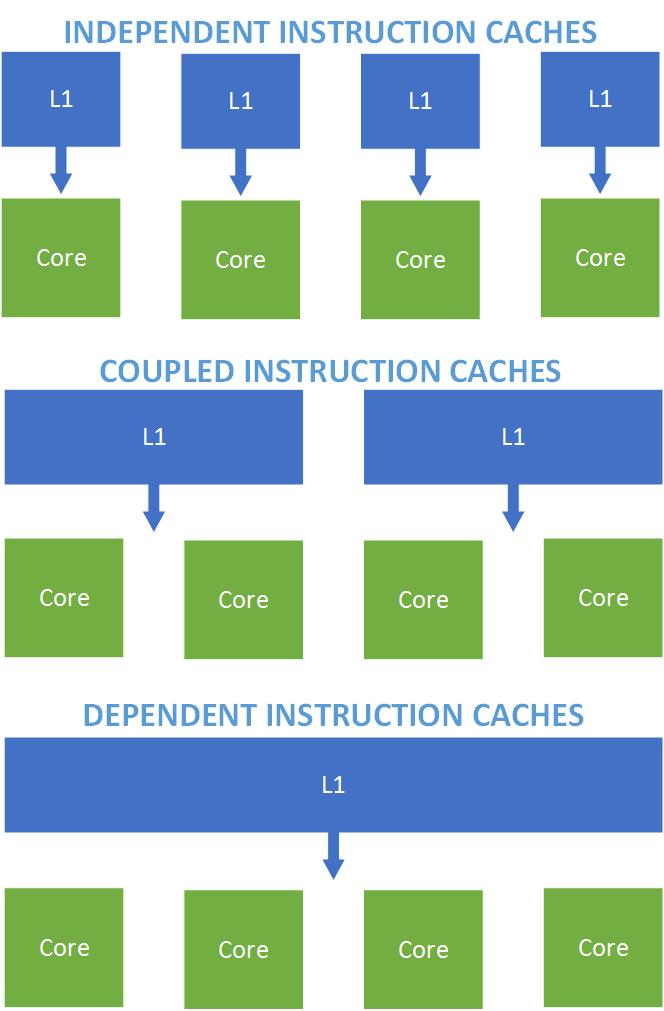
\includegraphics[width=90mm]{InstructionCacheDesignSketches.jpg}
\caption{(a) Current design of Instruction Caches in an SM, (b) Proposed cache design 1 (b) Proposed cache desgn 2.}
\label{propDesign}
\end{figure}

The architectural design associated with moden GPU's is one in which
each core in the GPU has access to its own instruction cache. 
Reducing the number of instruction caches for the same number of cores
in a streaming multiprocessor has certain advantages. 
First, using a shared instruction cache design we could reduce the
number of compulsory misses because an instruction previously executed
by one streaming multiprocessor may be available for another streaming
multiprocessor immediately rather than requiring an additional miss. 
We hypothesized that sharing an instruction cache would result in
increased efficiency and fewer cache misses. 
Figure~\ref{propDesign} shows the current design explaining the
interaction between GPUs and instruction caches, the proposed design
of sharing an instruction cache over multiple (but not all) cores in
the streaming multiporocessor and the last design ennumerates the
proposed design of a \emph{single} instruction cache to be shared by
all the cores on the steaming multiprocessor.
 




